\documentclass{article}
\usepackage{ctex}
\usepackage{graphicx}
\usepackage{amsmath}
\usepackage{indentfirst}
\usepackage{titlesec}
\usepackage{setspace}
\usepackage{subfigure}
\usepackage{caption}
\usepackage{float}
\usepackage{booktabs}
\usepackage{geometry}
\usepackage{multirow}
\geometry{left=1.2cm,right=1.2cm,top=2cm,bottom=2cm}
\title{\songti \zihao{2}\bfseries HW3反幂法求解矩阵按模最小特征值}
\titleformat*{\section}{\songti\zihao{4}\bfseries}
\titleformat*{\subsection}{\songti\zihao{5}\bfseries}
\renewcommand\thesection{\arabic{section}}
\author{王启骅 PB20020580}
\begin{document}
	\maketitle
	\section{实验结果与分析}
	\begin{figure}[!h]
		\centering
		\subfigure[$ A_1 $]{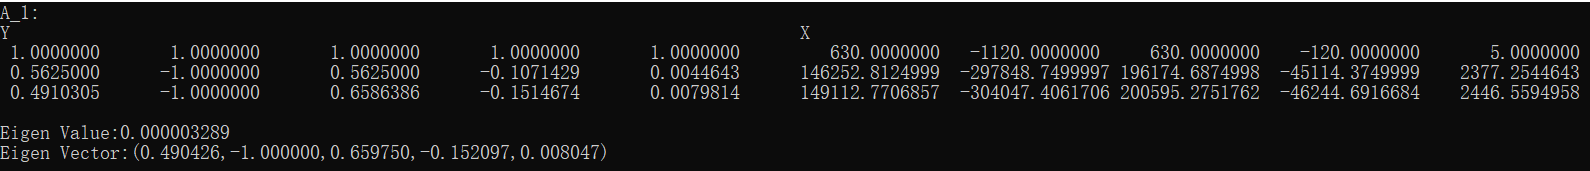
\includegraphics[scale=0.54]{result_A1}}
		\subfigure[$ A_2 $]{	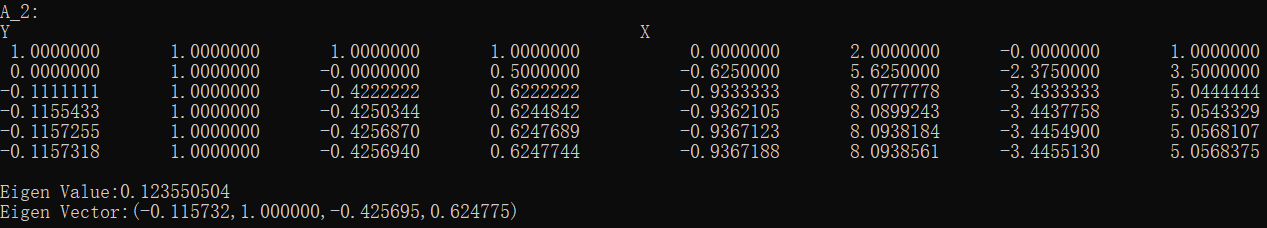
\includegraphics[scale=0.64]{result_A2}}
		\captionsetup{font={small},labelfont=bf}
		\caption{\heiti\zihao{-5}反幂法迭代结果}
		
	\end{figure}


$A_1$按模最小特征值为0.000003289,对应的特征向量(0.490426,-1.000000,0.659750,-0.152097,0.008047)。$ A_2 $的按模最小特征值为0.123550504,对应的特征向量(-0.115732,1.000000,-0.425695,0.624775)。


可见$ A_1 $迭代了3次,$ A_2 $迭代了6次。但是收敛速度应该不仅与按模最小的特征值的大小有关,还应该与其他特征值相对于最小特征值的大小有关。当按模最小的特征值相对于其他特征值远小时,在计算机允许的内存和精度范围内,是可以以更快的速度收敛。本次实验中全部矩阵是使用double型变量,暂未发现数值问题,但是分析可能出现的问题有例如按模最小特征值远比其他特征值小,导致数据精度难以达到,或者迭代过程中计算X值时可能因为数值过大溢出等。
\end{document}